% !TEX root = ../main.tex

\chapter{Introduction}
\label{ch:introduction}

\section{General Notation}
First, I am defining the notation I used throughout this thesis. For the scalars, I used regular, normal-weight variables such as $x$. Vectors are represented by bold lower-case variables like $\mathbf{x}$. Tensors and matrices are denoted by bold upper-case characters, such as $\mathbf{X}$. In summary:
\begin{align*}
x&: \text{Scalar} \\
\mathbf{x}&: \text{Vector} \\
\mathbf{X}&: \text{Matrix or tensor}
\end{align*}
\todo[inline]{Useful? Everything covered?}

\section{Reinforcement Learning Control Problems}
mention environment, reward \\ \\
In Reinforcement Learning (RL), we have an agent and an environment. The agent can take on actions to interact with the environment. The environment, on the other hand, always holds a certain state that can be altered by the actions of the agent. The goal of the agent is to learn a policy $\pi$ that drives the system into the desired state by taking the right actions. For example, the goal might be to solve skill games like Ball-in-a-Cup or Kendama (\cite{kober2010imitation}). However, we do not have data beforehand as we do in supervised learning problems. We only get a scalar reward signal that indicates how well the agent performs. The goal of the agent is to maximize the cumulative rewards received by the environment. Therefore, the agent needs to learn optimal behavior through trial-and-error interaction with the environment.
\begin{figure}[!ht]
\centering
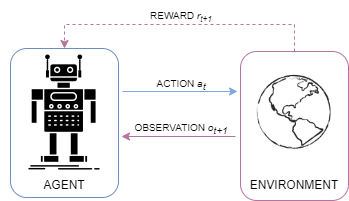
\includegraphics[width=.6\textwidth]{RL_agent_env}
\caption[Interaction loop between an RL agent and the environment]{
  \textbf{Interaction loop between an RL agent and the environment.}
  At timestep $t$, the agent receives the observation $o_t$ from the environment. The agent decides to select action $a_t$ and interacts with the environment. The enviornment changes and returns the next observation $o_{t+1}$ and the reward $r_{t+1}$ to the agent.
}
\label{fig:RL_agent_env}
\end{figure}
Figure~\ref{fig:RL_agent_env} illustrates the loop between the agent and the environment. The agent has received the observation $o_t$ from the environment and therefore knows the current state of it. The agent then performs some action $a_t$ in the environment. The environment changes according to the received action and returns an observation $o_{t+1}$ that indicates the current state of the environment and a reward $r_{t+1}$. One such interaction between the agent and the environment represents one \emph{timestep}.

The rewards correspond to an underlying reward function that is specific to the environment. The reward function is a function that maps the current state of the environment, the current action, and the subsequent state into a scalar value. The function can be deterministic or it can have a random component making it stochastic. Depending on the problem, the reward can be sparse or dense. Sparse reward means that the reward function returns zero in most of its domain and only returns a meaningful reward in a few rare settings or at the end of the experiment. That introduces a huge challenge since we cannot know which particular actions led to success or failure. Optimization problems with this setting are generally difficult. Dense reward environments return a meaningful reward at almost every time step.

Learning a policy that maximizes the returned rewards is generally non-trivial. The agent can only learn through trial and error. If the policy is not explorative enough, we might get stuck in a local optimum and never reach the goal. However, if there is too much exploration we loose reward. Thus, there needs to be a balance between exploration and exploitation. In addition, often there is a time delay for the reward. The consequence of an action might not be immediately visible to the agent. This problem is known as the credit-assignment problem in the literature (\cite{sutton2018reinforcement}).
\todo[inline]{Include MDP? Talk about sample efficiency? Talk about value function already? Talk about model-based and model-free?}

\section{Classic Reinforcement Learning}
Classic RL framework and approach \\ \\
We can solve RL problems with methods based on value functions or methods based on policy search. The value function is a prediction of future reward of landing on a specific state. It indicates how good or bad being in a certain state is. With methods based on value functions, the agent chooses the best action in the state. Methods based on policy search directly search for the optimal policy $\pi^*$ and do not need to maintain a value function model (\cite{8103164}).
\todo[inline]{Include Q-Learning, reward shaping? show more the difference between this and dps}

\subsection{Neural Networks as Models}
Neural networks are machine learning algorithms inspired by the functionalities of the human brain. They consist of connected neurons or nodes that imitate the biological neurons of the brain sending signals to each other. A neuron receives one or multiple input values and calculates one or multiple output values. Figure [insert figure] illustrates one neuron. The neuron receives three input values and calculates one output value. For the caluclation of the ouptut, the neurons uses the assigned weights $w$. Thus, the output represents the sum of weighted inputs.

In a neural network, the neurons are arranged in connected layers. A network has at least an input and an output layer. We can further expand it with one or more hidden layers. Depending on the model, the connectivity between the layers differs. Figure~\ref{fig:neural_network_sketch} shows a sketch of a network with three hidden layers that are fully connected.
\begin{figure}[ht]
\centering
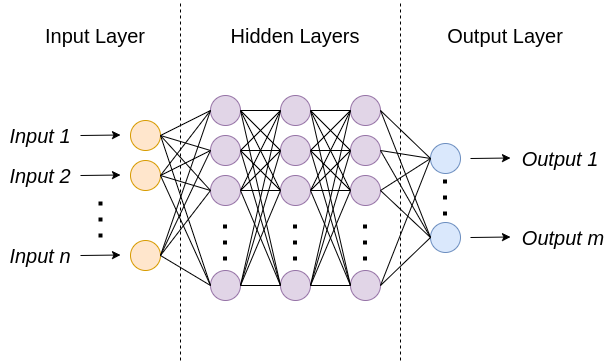
\includegraphics[width=.7\textwidth]{neural_network_sketch}
\caption[Sketch of a Neural Network]{
  \textbf{Sketch of a neural network.}
  The image shows a sketch of a neural network with three fully connected hidden layers. The network expects $n$ inputs and has $m$ possible outputs.
}
\label{fig:neural_network_sketch}
\end{figure}
Each neuron holds an associated weight and threshold. It receives an input and outputs the sum of weighted inputs. If this sum is greater than the associated threshold, the neuron gets activated.

A large part of the success of neural networks can be traced to the use of \textit{backpropagation}. Backpropagation uses information from the previous epoch (i.e. iteration) to adjust the weights of the network using the error gradient.

A neural network with one or more hidden layers defines a non-linear function. It is theoretically able to represent any function. Thus, neural networks are \textit{generic function approximators}. In addition, neural networks are highly expressive and flexible. They are applied successfully in many areas including in RL problems. Neural networks can be used to approximate a value function or a policy function. Deep RL combines RL with the methods from deep learning. It has been used in many applications including robotics, video games, computer vision (\cite{franccois2018introduction}).


%However, neural networks also come with a few limitations or disadvantages. The backpropagation algorithm requires the calculation of an accurate gradient. Depending on the problem, this can be a challenging task. For example, calculating an accurate gradient in RL problems is usually non-trivial. Furthermore, there is a lack of understanding. The output of a neural network is often incomprehensible because of its complex structure.

\todo[inline]{Should NN be explained in more detail? Write more about DRL, include recent results, advantages, disadvantages}

\section{OpenAI Gym}
\label{sec:gym}
mention as example of control problems, that it's a common benchmark in the literature, provides environments \\ \\
OpenAI Gym\footnote{https://www.gymlibrary.ml/} is a toolkit that provides environments that represent general RL problems. They are easy to use and serve as benchmark problems with varying difficulty and challenges.
\todo[inline]{Explain more, compare with Section~\ref{sec:environments} to not repeat}

\section{Direct Policy Search}
mention it as an alternative to Deep RL, mention it uses networks to approximate policy rather than value function \\ \\
An alternative to the methods described so far is direct policy search. Instead of approximating a value function, we approximate the policy directly with an independent function approximator with its own parametrization. Using a value function can work well but there are some limitations. Studies suggest that approximating a policy can be easier to use and deliver better results (\cite{sutton1999policy}; \cite{anderson2000approximating}).
Here we have two approaches: gradient-based and gradient-free methods.
\todo[inline]{Explain more, go more into advantages, find more papers with comparison}

\section{Neuroevolution}
special case of DPS: NN as policy approximator, train with evo \\ \\
Neuroevolution is a special case of direct policy search. A neural network is used to approximate the policy and optimized with evolutionary algorithms. It was shown that genetic algorithms can work well even in hard settings (\cite{such2017deep}).
\todo[inline]{Explain more}

\section{Black-Box Optimization}
but what is evo? here's a primer on black box optimization \\ \\
In Black-Box Optimization (BBO), the problem structure, as well as the model, remains unknown. BBO methods optimize a parametrization without any constraints on the problem, model or solution needed. Thus, there is no constraint on differentiability or convexity. The optimization is done solely based on a score or cumulative reward, which makes these methods directly applicable to Reinforcement Learning (RL) problems.
\todo[inline]{Explain more}

\subsection{Random Weight Guessing}
Randomization and RWG (uniform distribution) \\ \\
Random Weight Guessing (RWG) is the simplest BBO method. With RWG, we repeatedly randomly initialize the weights of a model until the resulting model classifies all training instances correctly. Then we test the model on a separate test set (\cite{schmidhuber2001evaluating}). RWG is not a reasonable learning algorithm, but it can be used as an analysis method (\cite{oller_analyzing_2020}).
\todo[inline]{Explain more, include limitations (expensive algorithms)}

\subsection{Evolution Strategies}
ES-(1+1) (normal, adapt mean) \\ \\
Evolution Strategies (ES) belong to the class of evolutionary algorithms and are best suited for continuous optimization. They are directly inspired by the idea of evolution in nature and use the concept of mutation and selection. ES are implemented in a loop where one iteration is called a generation. In each generation new individuals (candidate solutions) are generated using the current parents. We continue with the next generation until a stopping criteria is met. ES are multi-agent algorithms which means that they generate multiple parametrizations that explore a different path or area in the optimization space independently. This exploration prevents us from landing in a local optimum.

\textbf{(1 + 1)-ES:} The population model (1 + 1) means that we maintain only one individual. For the next generation, we generate one new offspring as a variation of the parent, drawn from the normal distribution. For this, we adapt the mean of the distribution according to the parent. Then we keep either the parent or the child based on which performed had a better fitness score. Algorithm~\ref{alg:ES} shows this process in pseudocode.
\begin{algorithm}
\caption{(1 + 1)-ES in $d$ dimensions}
\begin{algorithmic}[1]
\State Parameter: $\sigma > 0$
\State Initialization: $x = x_0 \in \mathbb{R}^d$
\While{not done}
    \State Sample $x' \sim \mathcal{N}(x, \sigma^2 I)$
    \If{$f(x') \leq f(x)$}
      \State $x \leftarrow x'$
    \EndIf
\EndWhile
\State Return $x$
\end{algorithmic}
\label{alg:ES}
\end{algorithm}

\todo[inline]{Explain more}


\subsection{Covariance Matrix Adaptation Evolution Strategy}
CMA-ES (which is a ES-(mu,lambda)) (normal, adapt mean, adapt covariance, large pop) \\ \\
Covariance Matrix Adaptation Evolution Strategy (CMA-ES) is a method for non-linear, non-convex optimization problems in continuous domain. For each iteration (generation), a population of new individuals is generated by sampling a multivariate normal distribution. After each iteration, the mean and the covariance matrix is updated (\cite{hansen2016cma}).

\todo[inline]{Include formulas from tutorial}

\section{Research Questions}
\label{sec:research_questions}
Start from the experiments. They are your answer. Which question do they answer? These are your research questions. \\
In the experiments section, mention explicitly which question each answers \\ \\
The main goal of this thesis is to compare alternative models to neural networks. To analyze and compare the different models and their architectures, I formulated the following research questions:
\begin{enumerate}
  \item How do function approximators other than neural networks compare with the latter?
  \item What impact has the bias on the performance of the model?
  \begin{enumerate}
    \item Does increasing the number of weights worsen the performance of the model?
    \item Does a neural network with more than two hidden layers yield worse scores?
    \item Does the neural network's performance suffer from an increase in the number of neurons?
    \item Does the difficulty of the environment affect the observed effect of the bias?
  \end{enumerate}
\end{enumerate}

\todo[inline]{Move to experiments? Or formulate questions concerning bias later? Maybe divide first question into multiple smaller ones.}
